\documentclass[11pt,letterpaper]{article}
\usepackage[utf8]{inputenc}
\usepackage[T1]{fontenc}
\usepackage[margin=1in]{geometry}
\usepackage{hyperref}
\usepackage{pdfpages}
\usepackage{fancyhdr}
\usepackage{graphicx}
\usepackage[french]{babel}

% Set up headers
\pagestyle{fancy}
\fancyhf{}
\fancyhead[L]{Carlos Denner dos Santos}
\fancyhead[R]{Application - Université de Sherbrooke}
\fancyfoot[C]{\thepage}

\hypersetup{
    colorlinks=true,
    linkcolor=black,
    urlcolor=blue,
    citecolor=black
}

% Fix for pandoc tightlist
\providecommand{\tightlist}{%
  \setlength{\itemsep}{0pt}\setlength{\parskip}{0pt}}

\begin{document}

% Title page
\begin{titlepage}
    \centering
    \vspace*{2cm}
    
    {\Huge\bfseries Application Package\par}
    \vspace{1cm}
    {\Large Poste de professeure ou professeur en gestion de l'intelligence artificielle\par}
    \vspace{0.5cm}
    {\large Offre 07823\par}
    \vspace{2cm}
    
    {\LARGE\bfseries Carlos Denner dos Santos\par}
    \vspace{1cm}
    
    {\large AI Scientist\par}
    {\large Montreal, QC, Canada\par}
    \vspace{0.5cm}
    {\large \href{mailto:carlosdenner@gmail.com}{carlosdenner@gmail.com}\par}
    {\large +1 (438) 836-4116\par}
    \vspace{2cm}
    
    {\large Département des systèmes d'information et méthodes quantitatives de gestion (SIMQG)\par}
    {\large École de gestion\par}
    {\large Université de Sherbrooke\par}
    \vspace{2cm}
    
    {\large\today\par}
\end{titlepage}

\clearpage

% Table of contents
\tableofcontents
\clearpage

% Include CV PDF (no section header, just the PDF itself)
\addcontentsline{toc}{section}{Curriculum Vitae}
\pagestyle{empty}
\includepdf[pages=-]{../data/latex/CarlosDenner_CV_resume.pdf}
\pagestyle{fancy}

\clearpage

% Letter of motivation
\section*{Lettre de motivation}
\addcontentsline{toc}{section}{Lettre de motivation}
Sherbrooke, le 17 novembre 2025

Objet : Candidature au poste de professeure ou professeur en gestion de
l'intelligence artificielle (offre 07823)

Madame, Monsieur,

Je vous soumets ma candidature au poste de professeure ou professeur en
gestion de l'intelligence artificielle (offre 07823) au Département des
systèmes d'information et méthodes quantitatives de gestion (SIMQG) de
l'École de gestion de l'Université de Sherbrooke.

Titulaire d'un doctorat en systèmes d'information au sein d'une faculté
de gestion, complété par des stages postdoctoraux en informatique et en
statistique, je travaille depuis plus de vingt ans à l'intersection de
l'analytique, des systèmes d'information et de la stratégie. Mes projets
récents portent sur la gouvernance et la régulation de l'IA, la gestion
de portefeuilles de projets d'IA, ainsi que sur l'ingénierie et
l'exploitation de systèmes d'IA à grande échelle, incluant des modèles
de type LLM et des systèmes de recommandation.

Sur le plan scientifique, j'ai publié notamment dans Ethics and
Information Technology (« Artificial Intelligence Regulation: a
framework for governance ») et dans Government Information Quarterly («
Artificial intelligence governance: Understanding how public
organizations implement it »). Ces travaux proposent, d'une part, un
cadre intégrateur pour la régulation de l'IA, et d'autre part, une étude
empirique de la mise en œuvre de la gouvernance de l'IA dans 28
organisations publiques sur cinq continents. Ils s'inscrivent
directement dans les thématiques du poste, en particulier la gouvernance
et la gestion des risques de l'IA ainsi que la sécurité et la résilience
des systèmes d'IA.

Parallèlement, j'ai conçu et déployé des systèmes analytiques et d'IA
dans des secteurs variés (télécommunications, énergie, santé, économie
sociale), ce qui me donne une vision très concrète des enjeux
d'AIOps/MLOps et de cycle de vie de l'IA en contexte organisationnel.
Mes recherches actuelles portent sur la sécurité des LLM (défense contre
la prompt injection, détection des hallucinations dans les systèmes
RAG), l'intelligence artificielle affective et les boucles affectives
dans l'interaction humain-LLM, ainsi que les théories de l'innovation
numérique (notamment le contrôle réversible). Ces travaux se traduisent
par des manuscrits pour MISQ, Academy of Management Review et
Communications of the ACM. J'ai récemment dirigé un projet de
cartographie de plus de 250 000 familles de brevets en apprentissage
automatique (2010--2025) afin d'identifier les domaines émergents liés à
la détection des hallucinations, à la défense contre la prompt
injection, à la sécurité des agents et à la fédéralisation de
l'entraînement de LLM. Ce travail illustre ma manière de faire : croiser
rigueur analytique, compréhension fine des organisations et
préoccupations stratégiques.

Le programme de recherche que je propose s'articule autour de trois axes
: (1) la gouvernance et la gestion des risques des systèmes d'IA dans
les organisations ; (2) l'ingénierie, les opérations et la sécurité des
systèmes d'IA (AIOps/MLOps) avec un focus sur la sécurité des LLM
(prompt injection, hallucinations), les systèmes agentiques et l'IA
affective ; et (3) la performance, l'impact et la durabilité de l'IA en
contexte organisationnel. L'objectif est de produire à la fois des
contributions théoriques (théories de l'innovation numérique, modèles de
gouvernance, cadres d'évaluation de la sécurité des LLM, théories des
boucles affectives) et des outils directement utiles aux organisations
(référentiels de défense contre la prompt injection, patrons
d'architecture pour systèmes RAG sécurisés, tableaux de bord, cas
d'enseignement), en forte synergie avec le SIMQG, le Centre de recherche
Createch sur les organisations intelligentes (CROI) et le Centre Laurent
Beaudoin.

En enseignement, j'ai une expérience significative à tous les cycles
dans des cours de systèmes d'information, d'analytique d'affaires, de
transformation numérique et de gouvernance de l'IA. Ma philosophie est
de partir de problèmes réels, d'outiller les étudiantes et étudiants
pour les structurer grâce aux données et aux modèles, puis de les amener
à réfléchir aux implications organisationnelles et sociétales de leurs
solutions. L'orientation pratique et partenariale de l'École de gestion
correspond très bien à cette approche.

Enfin, je suis particulièrement attiré par la culture de collaboration
interdisciplinaire et par l'accent mis sur la formation de leaders
capables de diriger la transformation numérique s'appuyant sur l'IA. Je
serais heureux de m'investir pleinement dans les projets du SIMQG, du
CROI et de l'École de gestion, en recherche, en enseignement et en
service à la collectivité.

Je vous remercie de l'attention portée à ma candidature et me tiens à
votre disposition pour toute information complémentaire.

Veuillez agréer, Madame, Monsieur, l'expression de mes salutations
distinguées.

Carlos Denner dos Santos carlosdenner@gmail.com +1 (438) 836-4116


\clearpage

% Research program
\section*{Programme de recherche}
\addcontentsline{toc}{section}{Programme de recherche}
Programme de recherche Gestion, gouvernance et ingénierie des systèmes
d'intelligence artificielle

Depuis plus de vingt ans, je travaille à l'intersection des systèmes
d'information, des données et de la gestion. Avec l'essor de l'IA, et en
particulier des modèles de type LLM et des systèmes agentiques, la
question centrale pour les organisations n'est plus ``que peut-on faire
avec l'IA ?'', mais ``comment la gouverner, l'exploiter et la sécuriser
de façon responsable, performante et durable ?''.

Le programme de recherche que je propose à l'Université de Sherbrooke
vise précisément ce point. Il se structure en trois axes complémentaires
:

\begin{enumerate}
\def\labelenumi{\arabic{enumi}.}
\tightlist
\item
  Gouvernance et gestion des risques de l'IA dans les organisations
\item
  Ingénierie, opérations et sécurité des systèmes d'IA (AIOps/MLOps),
  avec un focus sur les LLM et agents
\item
  Performance, impact et durabilité de l'IA en contexte organisationnel
\end{enumerate}

Ces axes s'inscrivent directement dans les thématiques du poste
(gouvernance et risques, AIOps/MLOps, sécurité et résilience,
performance des systèmes d'IA) et dans la mission du Département des
systèmes d'information et méthodes quantitatives de gestion (SIMQG), au
cœur de la transformation numérique, de l'analytique et de la
cybersécurité.

Je m'appuie sur trois blocs d'expérience : -- un ancrage académique en
systèmes d'information et gouvernance de l'IA, avec des publications
dans des revues à comité de lecture (notamment Ethics and Information
Technology et Government Information Quarterly) ; -- une pratique
terrain de projets d'IA et d'analytique dans les télécommunications,
l'énergie, la santé et le secteur public ; -- un travail récent de
cartographie de plus de 250 000 familles de brevets en IA/ML
(2010--2025) pour identifier les domaines émergents liés à la
gouvernance, la sécurité et l'ingénierie de l'IA.

Axe 1 -- Gouvernance et gestion des risques de l'IA

Dans l'article « Artificial Intelligence Regulation: a framework for
governance » (Ethics and Information Technology, 2021), coécrit avec des
collègues, nous proposons un cadre intégrateur pour la régulation de
l'IA à l'échelle des politiques publiques. Dans « Artificial
intelligence governance: Understanding how public organizations
implement it » (Government Information Quarterly, 2025), nous analysons
comment 28 organisations publiques sur cinq continents traduisent (ou
non) ces principes dans leurs pratiques.

Le premier axe prolonge ces travaux au niveau organisationnel et des
portefeuilles d'IA, avec un accent particulier sur les risques émergents
liés aux LLM et aux systèmes agentiques. Les questions centrales sont :

-- Comment les organisations structurent-elles la gouvernance de leurs
systèmes d'IA (rôles, comités, politiques, processus de décision) ? --
Quels modèles de gouvernance (centralisé, fédéré, par domaine
d'affaires) sont les plus adaptés selon le secteur et la maturité
numérique ? -- Comment cartographier de manière exploitable les risques
liés à l'IA (biais, non-conformité réglementaire, cyberrisques
spécifiques aux LLM comme la prompt injection et les hallucinations,
dépendance à des fournisseurs, perte de contrôle sur des agents
autonomes, boucles affectives incontrôlées dans les systèmes d'IA
conversationnelle) pour aider les gestionnaires à prioriser ? -- Comment
les organisations peuvent-elles implémenter un « contrôle réversible »
permettant d'ajuster dynamiquement leurs systèmes d'IA tout en
maintenant des capacités d'apprentissage organisationnel ?

Je prévois de combiner études de cas approfondies, entretiens, analyse
de documents et enquêtes quantitatives. L'objectif est de produire : --
des typologies de structures de gouvernance de l'IA ; -- des cartes de
risques et de contrôles associés ; -- des guides pratiques et cas
d'enseignement utilisables dans les programmes de l'École de gestion
(dont le microprogramme de 3e cycle en gestion stratégique de l'IA et
l'École d'été en gestion stratégique de l'IA).

Axe 2 -- Ingénierie, opérations et sécurité des systèmes d'IA
(AIOps/MLOps)

Le deuxième axe se concentre sur le cycle de vie des systèmes d'IA :
données, modèles, déploiement, exploitation, monitoring, sécurité. C'est
le cœur de l'AIOps/MLOps, là où les enjeux de gouvernance se
matérialisent vraiment. Mes travaux récents portent spécifiquement sur
la sécurité des LLM et les dimensions affectives de l'interaction
humain-IA.

Les questions de recherche incluent :

-- Comment concevoir des pipelines AIOps/MLOps ``gouvernables'', où
traçabilité, contrôles d'accès, revues de risques, audits et mécanismes
d'arrêt (``kill switches'') font partie de l'architecture et des outils,
plutôt que de rester dans des documents ? -- Quels patrons
d'architecture pour les systèmes basés sur des LLM (RAG, agents, chaînes
d'outils) permettent de garder la main sur ce que le système peut faire,
sur quelles données et avec quelles garanties ? -- Comment intégrer la
sécurité (prompt injection, hallucinations critiques, exfiltration de
données, agents sur-permissionnés) dans les pratiques MLOps, au même
titre que la performance et la disponibilité ? -- Comment construire un
``pare-feu LLM'' (LLM Firewall) avec des défenses multi-phases contre la
prompt injection, depuis l'analyse de brevets jusqu'aux garde-fous
déployables côté entrée ? -- Comment évaluer et atténuer les
hallucinations dans les systèmes de génération augmentée par
récupération (RAG) ? -- Comment les boucles affectives émergent-elles
dans l'interaction humain-LLM, et quelles implications ont-elles pour la
conception des systèmes d'IA conversationnelle et l'analyse de sentiment
?

Sur ce volet, je m'appuie sur : -- des projets industriels concrets (par
exemple un système d'optimisation énergétique pour un grand opérateur
télécom, un système de recommandation IA pour l'application Jooay
favorisant l'inclusion numérique des enfants et jeunes en situation de
handicap, des projets de transformation numérique dans le secteur
public) ; -- un travail systématique sur les brevets en IA/ML montrant
que la détection d'hallucinations, la défense contre la prompt
injection, la sécurité des agents et la fédéralisation de l'entraînement
des LLM sont des domaines émergents où l'activité reste faible au regard
des enjeux ; -- des manuscrits en préparation pour des revues de premier
plan : « Building an LLM Firewall » (Communications of the ACM), «
Evaluating and Mitigating Hallucinations in RAG » (cadre expérimental),
« LLMs, Sentiment Analysis, and Algorithmic Feelings » (Academy of
Management Review), et « Reversible Control as a Digital Innovation
Theory » (MISQ Theory \& Review).

Je privilégierai des approches de design science et de recherche
orientée artefact : conception et évaluation de prototypes de pipelines
MLOps intégrant des points de contrôle de gouvernance, d'\,``agents
firewall'' encadrant ce qu'un agent LLM peut faire, de systèmes RAG avec
atténuation des hallucinations, et de tableaux de bord de risques et de
performance opérationnelle. Ces artefacts seront développés et évalués
avec des organisations partenaires (secteur public, télécom, énergie,
santé), en visant à la fois des contributions scientifiques (théories,
modèles, taxonomies, cadres d'évaluation) et des livrables directement
utilisables.

Axe 3 -- Performance, impact et durabilité de l'IA

Le troisième axe répond à une question que je rencontre régulièrement :
l'IA crée-t-elle réellement de la valeur, pour qui et à quel coût ? Il
s'agit ici de passer des promesses et des preuves de concept à une
évaluation rigoureuse de la performance, de l'impact et de la durabilité
des systèmes d'IA.

Les questions de recherche sont, par exemple :

-- Comment définir et mesurer la performance de projets d'IA au-delà des
métriques techniques (précision, F1) : valeur économique, qualité de
service, impact sur les processus, équité, effets sur le travail humain
? -- Quels facteurs distinguent les projets qui passent à l'échelle de
ceux qui restent au stade de pilote (alignement stratégique, maturité
des données, structures de gouvernance, capacités AIOps/MLOps,
acceptation des utilisateurs) ? -- Comment intégrer la durabilité
(environnementale, économique, sociale) dans la priorisation et
l'évaluation des portefeuilles d'IA ?

Je prévois des études de cas longitudinales (avant / après,
quasi-expériences, analyses de séries temporelles) combinées à la
construction de tableaux de bord de performance co-conçus avec des
partenaires. Les résultats nourriront directement les formations de
l'École de gestion destinées aux gestionnaires et aux professionnelles
et professionnels en exercice.

Approche, environnement et formation

Globalement, mon programme de recherche est pluridisciplinaire et
multi-méthodes : ancré en systèmes d'information et en gestion de la
technologie, combinant méthodes qualitatives, quantitatives et de
design, et toujours connecté à des organisations réelles.

Le SIMQG, au cœur de la transformation numérique, de l'analytique et de
la cybersécurité, est un environnement idéal pour développer ce
programme en lien avec le Centre de recherche Createch sur les
organisations intelligentes (CROI) et le Centre Laurent Beaudoin. Les
projets envisagés se prêtent bien à des demandes de financement au CRSH,
au FRQSC, à Mitacs et à des partenariats publics et privés.

Pour les étudiantes et étudiants de maîtrise, de doctorat et des
microprogrammes de 3e cycle, ce programme offre un terrain riche pour
des travaux qui combinent analyse rigoureuse, développement d'outils ou
de méthodes, et impact concret dans les organisations. À horizon cinq
ans, l'objectif est que l'École de gestion de l'Université de Sherbrooke
soit reconnue comme un pôle de référence pour la gestion stratégique, la
gouvernance et l'ingénierie des systèmes d'IA, au Québec et à
l'international.


\clearpage

% Teaching statement
\section*{Énoncé d'enseignement}
\addcontentsline{toc}{section}{Énoncé d'enseignement}
\input{enonce_enseignement_content.tex}

\clearpage

% Key publications
\section*{Three Key Publications}
\addcontentsline{toc}{section}{Three Key Publications}

\subsection*{Publication 1: Artificial intelligence governance}
\addcontentsline{toc}{subsection}{AI Governance (Government Information Quarterly)}
\pagestyle{empty}
\includepdf[pages=-]{Publications/1-s2.0-S0740624X24000959-main.pdf}
\pagestyle{fancy}

\subsection*{Publication 2: Artificial Intelligence Regulation}
\addcontentsline{toc}{subsection}{AI Regulation Framework (Ethics and Information Technology)}
\pagestyle{empty}
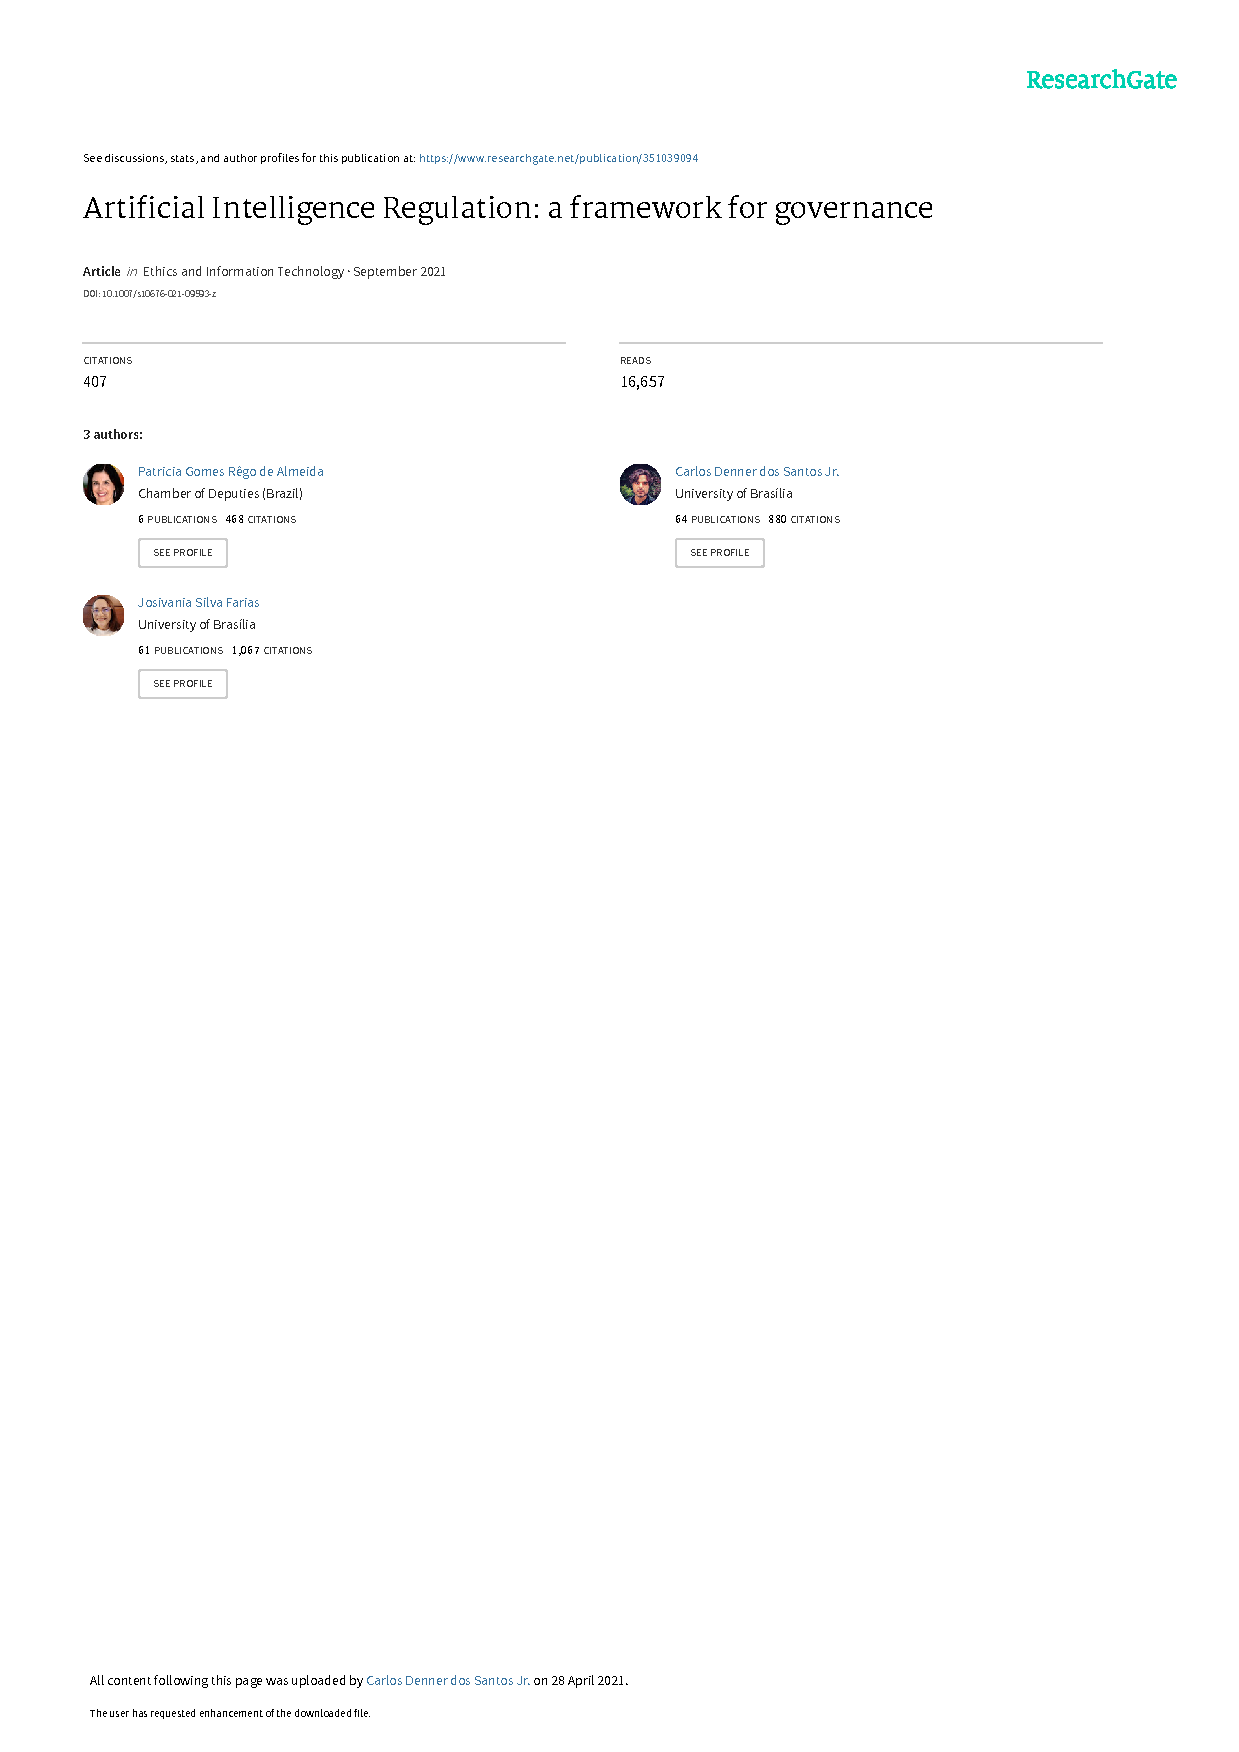
\includepdf[pages=-]{Publications/Almeida2021_Article_ArtificialIntelligenceRegulati.pdf}
\pagestyle{fancy}

\subsection*{Publication 3: The Attraction of Contributors in FOSP}
\addcontentsline{toc}{subsection}{Open-Source Contributors (MIS Quarterly)}
\pagestyle{empty}
\includepdf[pages=-]{Publications/TheAttractionofContributorsinFOSP.pdf}
\pagestyle{fancy}

\end{document}
